\label{sec:nonparametric:truncation}
\researchBasedOn[This section]{Lumori2014TIM}
%TODO: {labels into standardized form}

% This section uses nonparametric models in conjunction with the \gls{LPM}~\citep{Pintelon2010LPM1} to estimate the complex-valued \gls{FRF} in a linear \gls{LS} fashion.
% The advantage of using the nonparametric models is basically that the `models` often are very simple and hence require little user interaction to construct.
% Among the current nonparametric methods, the \gls{LPM} method is chosen due to its superiority over the classical nonparametric methods (windowing) in suppressing leakage errors~\citep{Bendat1993,Oppenheim1983,Schoukens2006LPM}. 
% Consequently, the \gls{LPM} estimate of the \gls{FRF} is not hampered by leakage errors \citep{Pintelon2010LPM1,Schoukens2009LPM}. 
% Note that a more general discussion on the \gls{LPM}, applied to noisy, real-valued data is found in \citep{Fan1996} with a specific focus on parametric tuning.

The main contribution of this section is to come up with an improved \gls{FRF} by developing a method for smoothing the \gls{FRF} estimated via the \gls{LPM}. 
The smoothing of the \gls{FRF} happens by truncating the associated impulse response, as in~\citet{Schoukens1998}, but with the following additional extension: the determination of the optimal truncation time, without any user interaction, in conjunction with the use of the \gls{LPM} for leakage reduction. 
The truncation point (cut-off index) is determined by one of two statistically inspired methods.
It is then shown that a smooth \gls{LPM} estimate of the \gls{FRF} lowers the variance, thus improving the assessment level of the dynamic properties of a given \gls{LTI} system.
It should be noted, however, that such smoothing is merely of importance when inspecting the \gls{FRF} visually.
In particular, a slight bias might be incurred when smoothing the \gls{FRF}.
If one is to fit a parametric model to the smoothed \gls{FRF}, one essentially ends up with a biased model (which is often undesirable).

Based on \citet{Schoukens2009LPM}, the nonparametric method developed in this work is formulated in an \gls{OE} framework. 
A \gls{SISO} \gls{LTI} system is considered.
The input signal is a known random noise signal and the output signal is corrupted by measurement noise. This is depicted in \figref{fig:nparam:blockH0} as a linear dynamic discrete-time \gls{SISO} system, whose full mathematical model is of the form:
\begin{equation}\label{eq:nparam:trunc:LPM:TD}
y(t)=G_0(q)u_0(t)+H_0(q)e(t)=G_0(q)u_0(t)+v(t)
\end{equation}
where $G_0(q)$ represents the dynamics of the system to be estimated, $u_0(t)$ is the input signal, $v(t)= H_0(q)e(t)$ is the noise source at the output, $H_0(q)$ is the noise dynamics, $e(t)$ is white noise, and $q^{-m}$ is the backwards shift operator ($q^{-m}x(t)$ = $x(t-m)$  with $m$ a positive integer).

Numerous parametric identification techniques are devoted to the development of parametric plant $G(q,\theta)$ and noise models  $H(q,\theta)$, where  $\theta$ is the model parameters vector~\citep{Ljung1999,Soderstrom1989}. 
In this section, however, a nonparametric technique is developed, and formulated in the frequency domain, consistent with \citep{Pintelon2012,Mahata2006}. 

The following  choices are made:

\begin{itemize}

\item The work in this section is for discrete-time systems. 
Denote the $k^{\text{th}}$ discretized frequency as $\omega_k$ = $e^{-j2{\pi}k\fs/N}$, with $\fs$ the sample frequency and $N$ the total number of sample points.

\item  Describe the parametric plant model  $G(q,\theta)$ by the nonparametric \gls{FRF} counterpart  $G(\omega_k)$  at the $k^{\text{th}}$ frequency.

\item Describe  the parametric noise model $H(q,\theta)$ (associated with the output noise source $v(t)$) by a nonparametric noise variance contribution $\sigma^2_v(\omega_k)$ at the $k^{\text{th}}$ frequency.

\end{itemize}

The rest of the section is structured as follows. 
\secref{sec:nparam:trunc:smoothingFRFestimate} discusses the novel smoothing method.
Ultimately, in \secref{sec:nparam:trunc:simResults}, simulation results of the following \gls{FRF} estimates and their corresponding variances are compared: (i) the smooth \gls{LPM} estimate $\hat{G}_{\trunc}(\omega_k)$, (ii) the \gls{LPM} estimate $\hat{G}_{\LPM}(\omega_k)$.

These \gls{FRF} estimates are also compared with the true \gls{LTI} system ${G}_0(\omega_k)$.
Discussion of the simulation results is then followed by a conclusion in \secref{sec:nparam:trunc:conclusion}.

% \begin{assumption}
% The spectrum of the  input signal $U_0$ is not a smooth function of the frequency, but a rough function, i.e. $U_0(k+1) - U_0(k)$ should not vanish to zero~\citep{Schoukens2009LPM}.
% \end{assumption}

% In other words, for the excitation signal to be rough: the magnitude of the spectral difference $|U_0(k+1) - U_0(k)|$ must have a probability of 1 (unity) for it to remain in the same order of magnitude as $|U_0(k)|$, irrespective of the record length $N\rightarrow\infty$ and the corresponding  frequency resolution $f_0\rightarrow{0}$.

% \begin{assumption}
% The measured output signal is $y(t) = y_0(t) + v(t)$ with the exact input signal $u_0(t)$ known. 
% The filtered white noise $v(t) = H_0(q)e(t)$ is the disturbing noise source at the output.
% \end{assumption}


% \subsubsection{The Hanning Window and the \glsentrytext{LPM}}
% \label{sec:nparam:trunc:LPMFRFest}
% \paragraph{Windowing}
% The effect of windowing may be  exemplified by use of the Hanning window, which is a popular choice.
% In a nutshell, the Hanning window is effective in reducing  the leakage errors, but  with a trade off of increased interpolation errors. 
% Pertinent details of the Hanning window are discussed in \citep{Schoukens2006LPM,Antoni2007FRF,Schoukens2009LPM,Wellstead1981} and \citep{Harris1978}.

% The anomalies due to interpolation errors, associated with windowing, can easily be mitigated or circumvented by use of the \gls{LPM}. 
% As shown in \citep{Pintelon2012}, the leakage errors are reduced from  $\bigO{{N}^{-1}}$, for Hanning windowing, to $\bigO{{N}^{-3}}$ or better, for the \gls{LPM}.

% \paragraph{Formulation of the Linear LS LPM}
% The \gls{LPM} is formulated as a nonparametric local linear \gls{LS} estimate using the full data record of length $N$ as outlined below \citep{Schoukens2009LPM}.
% \citet[Section 7.2.2]{Pintelon2012} gives the general formulation of the \gls{LPM} for \gls{MIMO} systems.
% The formulation in this section is a summary for a \gls{SISO} system.

% The \gls{DFT} spectra at the output of the \gls{SISO} system in \figref{fig:nparam:blockH0} are derived from equations \eqref{eq:nparam:trunc:LPM:TD} and \eqref{eq:nparam:trunc:LPM:leakage}, \latin{viz}:
% \begin{equation}\label{lpm1spectra}
% Y(k)=G_0(\omega_k)U_0(k)+T(\omega_k)+V_0(k)
% \end{equation}
% where $V_0(k) = H_0(\omega_k)E(k)$ is a noise term, and $T(\omega_k)$ is the leakage term. The latter is the sum of the system and the noise leakage terms, i.e. $T(\omega_k) = T_G(\omega_k) + T_H(\omega_k)$.

In this section, the $\lpm{3,2,2}$ is used.
However, since the techniques discussed in this section are not specifically geared towards the \gls{LPM}, one can just as well use the concepts with other non-parametric \gls{FRF} estimators such as the \gls{LRM}.

\subsection{Smoothing the \glsentryshort{FRF} estimate}
\label{sec:nparam:trunc:smoothingFRFestimate}
The method for smoothing (improving) the \gls{LPM} estimate of the frequency response function  is presented in this section together with pertinent assumptions.
After obtaining the \gls{LPM} estimate of the \gls{FRF} (denoted as $\hat{G}_{{\LPM}}(\omega_k)$) from \secref{sec:nparam:LPM}, the smoothing method is decomposed into the following procedures (see \figref{fig:nparam:truncation:workflow}), which will be elaborated on later:
\begin{enumerate}
\item The impulse response $\hat g_{\LPM}(t)$  is computed from the \gls{IDFT} of $\hat{G}_{{\LPM}}(\omega_k)$.

\item An accurate estimate of the \gls{DC} value of the \gls{FRF} is computed by inspecting the average value of the tail of the estimated impulse response and this is subtracted from the impulse response.

\item From the estimated impulse response $\hat{g}(t)$, the noise floor is estimated.

\item Assuming that the impulse response decays with the passing of time, the noise is bound to predominate after a certain time interval. 
In particular, when $t > \truncTime$, the impulse response has decayed below the noise floor.
In \secref{sec:nonparametric:truncation:ftest} and \secref{sec:nonparametric:truncation:exponentialfit}, two approaches are introduced to estimate $\truncTime$.

\item A truncation is effected at the point beyond which the estimated impulse response is buried in noise.
This action results in smoothing of the \gls{FRF} when the truncated impulse response is transformed to the frequency domain using the \gls{DFT}.
\end{enumerate}

\begin{figure}
   \centering
   \setlength{\figurewidth}{0.75\columnwidth}
   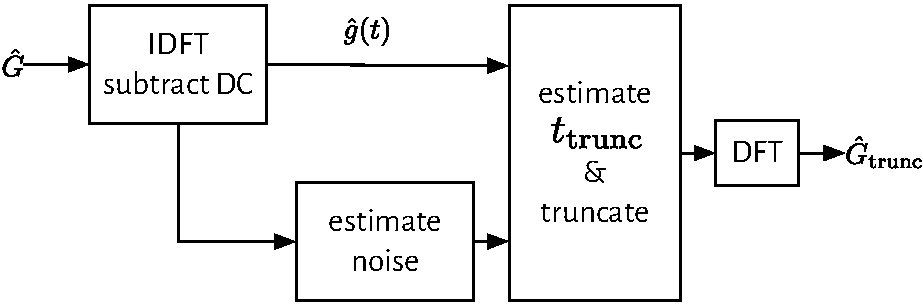
\includegraphics[width=\figurewidth]{\thisDir/figs/workflow-truncation.pdf}
   \caption{Workflow for impulse response truncation.}
   \label{fig:nparam:truncation:workflow}
 \end{figure} 

These procedures require that the following assumptions are satisfied.

\begin{assumption}
The estimate $\hat G_{\LPM}(\omega_k)$ is available at all frequencies $\omega_k$ for $k\in\{1,2,\dots,N/2\}$.
\end{assumption}

This assumption ensures that the impulse response corresponding to the \gls{FRF} can be computed (up to its mean value). It requires that the input signal excites the whole unit circle. This is satisfied, for instance, by using white noise as an excitation signal.


\begin{assumption}\label{ass:imprespdecay}
The impulse response $g(t)$ decays exponentially over time, i.e. 
\[
  \exists A \in \PositiveRealNumbers, 
  \exists a > 0 ,
  \exists t_0 > 0,
  \forall t > t_0: 
     \abs{g(t)} \leq A \exp(- a t) \text{.}
\]
\end{assumption}

\begin{assumption}\label{ass:decay90perctime}
Within $90\%$ of the measurement window, the impulse response decays
 to a level that is indistinguishable from the noise.
\end{assumption}

Note that \assref{ass:imprespdecay} and \assref{ass:decay90perctime} exclude the possibility of considering a system that is a pure integrator.

\subsection{Obtaining the Impulse Response Function}

The estimated impulse response function  $\hat g_{{\LPM}\setminus \mathrm{DC}}(t)$ is obtained explicitly via the \gls{IDFT} of the \gls{LPM}-estimate $\hat G_{\LPM}(\omega_k)$ of the \gls{FRF}, \latin{viz}:
\begin{align}\label{eq:impRespiDFT}
\hat g_{{\LPM}\setminus \mathrm{DC}}(t) 
&= 
\frac{1}{\sqrt{N}}
\sum_{k=1}^{N-1}
\hat G_{\LPM}(\omega_k)e^{\frac{j2\pi kt}{N}}
\end{align}
where the estimated \gls{FRF} in the frequency band between  the Nyquist and the sample frequencies is obtained as follows:
\begin{align}
\hat G_{\LPM}(\omega_{N-k}) = \overline{\hat G_{\LPM}(\omega_k)},\ \text{for}\ k=1,\dots,N/2
\end{align}
(with $\conj{\hat G_{\LPM}}$ the complex conjugate of $\hat G_{\LPM}$) to ensure $\hat g_{\LPM}(t)$ to be real.

Smoothing of the estimated \gls{FRF} requires the correct estimate of the impulse response. 
Unfortunately, the \gls{LPM} presented in \secref{sec:nparam:LRM} and in \citep{Schoukens2009LPM} does not estimate the \gls{DC} value of the \gls{FRF}, hence the subscript ``$\setminus\mathrm{DC}$'' in equation \eqref{eq:impRespiDFT}. 
Consequently, the mean value of the corresponding estimated impulse response given in equation \eqref{eq:impRespiDFT} is not correct. 
This limitation is lifted by developing a simple estimator of the mean value, presented below.

\subsection{Estimating the \glsentrytext{DC} Value of the \glsentrytext{FRF}}\label{sec:nparam:trunc:DCvalueEst}
The correct mean value of the impulse response accounts for (i.e. estimates) the \gls{DC} value of the \gls{FRF}. A time-domain method is proposed for estimating the mean value of the impulse response in equation \eqref{eq:impRespiDFT}. %The first is a frequency-domain technique and the second is a time-domain technique.

According to \assref{ass:imprespdecay}, the true impulse response tends to zero asymptotically; and by \assref{ass:decay90perctime}, the last $10\%$ of the estimated impulse response is noise, plus a constant value due to an inaccuracy in the    average value of the impulse response. The correct estimate of the mean value is obtained by shifting the whole signal such that the last $10\%$ of the impulse response is centered around 0.
To this end, the following procedure is executed:


\begin{enumerate}
\item Compute the mean value $m_{g10}$ of the last 10\% of the impulse response $\hat g_{{\LPM}\setminus \mathrm{DC
}}(t)$, estimated by the \gls{LPM}, as %$\hat g_{\LPM}(t)$ as
\begin{align}
   m_{g10} 
   = 
   \frac{1}{\lceil0.1N - 1\rceil}
   \sum_{t=\lfloor0.9N\rfloor}^{N-1}
      \hat g_{{\LPM}\setminus \mathrm{DC}}(t)
\end{align}

\item Next, subtract the computed mean value $m_{g10}$ from $\hat g_{{\LPM}\setminus \mathrm{DC
}}(t)$ to obtain the improved impulse response $\hat g_{\LPM}(t)$, \latin{viz}:
\begin{align}
\hat g_{\LPM}(t) = \hat g_{{\LPM}\setminus \mathrm{DC}}(t) - m_{g10},\ \text{for}\ t=0,1,\dots,N-1
\end{align}
\end{enumerate}

\subsection{Determining the Truncation Time}
In this section, two methods will be discussed to determine the truncation time, i.e. the time beyond which the measured impulse response cannot be separated from the noise level.
Specifically, the first method uses an $F$-test to distinguish between signal and noise.
The second method fits an exponential through a well-chosen subset of the data to obtain $\truncTime$. 

\subsubsection{Truncation Via the $F$-Test}
\label{sec:nonparametric:truncation:ftest}
To distinguish the part of the measured impulse response where the actual impulse response dominates from the part where the noise dominates, the estimated impulse response $\hat{g}_{\LPM}$ is split into smaller segments. 
One can then gradually determine if in each of these segments, the observed impulse response is dominated by the noise.

% 1) cut into NS segments of minimally NM samples
% 2) assume last segment == noise
%    start from back
% 3) F-test on Var, Var==RMS if dc == 0 (i.e. noise)
%    H0: s²(1) =  s²(2)
%    H1: s²(1) >  s²(2)
%    alpha >> ==> beta <<
% 4) if H1 and RMS(signal)/RMS(noise) < f
%    robustness, SNR
%    select segment i
% 5) refine until wanted resolution is obtained

\begin{enumerate}
  \item The impulse response $\hat{g}_{\LPM}(t)$ is split into $N_S$ segments of approximate equal lengths
$L_S = \floor{\frac{N}{N_S}}$. 
If necessary, the length of the first segment is reduced to allow for the others to have equal lengths.
The $i^{\text{th}}$ segment is denoted $\segm{\hat{g}}{i}$, for $i \in \left\{1,\ldots,N_S\right\}$.
  By \assref{ass:decay90perctime}, the last segment, $\segm{\hat{g}}{N_S}$, is noise when $L_S \leqslant 0.1N$.
  
  \item Iteration is then carried out from the last segment ($i = N_S$) towards the beginning of the impulse response. To determine whether the preceding segment $\segm{\hat{g}}{i-1}$ is completely dominated by noise,  both an $F$-test and an absolute criterion on the RMS are used.

  The $F$-test is suited to compare the variances of different segments $\segm{\hat{g}}{i}$ and $\segm{\hat{g}}{i-1}$ \citep{Parsons1974}, while accounting for the degrees of freedom in each segment.
  For zero-mean noise, these variances are the \gls{RMS} value of each noise segment.
  This has the advantage that a segment in which the impulse response still has a significant amplitude is likely to have a large \gls{RMS} value, which is more likely to be detected.
  Let $s^2(i)$ denote the mean square value of segment $\segm{\hat{g}}{i}$, \latin{viz}:
  \begin{equation}
    s^2(i) 
    \isdef \frac{1}{L_S} \sum_{j=1}^{L_S} \left(\segm{\hat{g}}{i}(j)\right)^2
    = \left( \rms{\hat{g}^{[i]}} \right)^2
           \text{.}
  \end{equation}
  Starting with the last segment ($i = N_S$), the following null hypothesis and the alternative hypothesis are formulated:
  \begin{align}
     \nullHypothesis &: s^2(i-1) = s^2(i)\\
     \altHypothesis    &: s^2(i-1) > s^2(i)
     \text{.}
  \end{align}
  As segment $\segm{\hat{g}}{i}$ has been tested and been classified as noise (or assumed to be noise if $i=N_S$), the null hypothesis effectively states that the segment $\segm{\hat{g}}{i-1}$ is also noise.
  The alternative case occurs when $\segm{\hat{g}}{i-1}$ has a significant change, which indicates the presence of the signal.
  Using the $F$-test on the \gls{RMS} values of the two segments with a high confidence level of $\alpha=0.999$ and the aforementioned hypotheses, we can determine whether $\segm{\hat{g}}{i-1}$ is likely to be part of the actual impulse response.
  In particular, the null hypothesis is rejected when the empirical $F$ statistic is high, i.e.
  \begin{equation}
    F \isdef \frac{s^2(i-1)}{s^2(i)} \geq \ICDF{\FDistribution} \left( \alpha; n_{i-1}, n_{i} \right)
  \end{equation}
  where $ \ICDF{\FDistribution}$ is the inverse \gls{CDF} of the \mbox{$F$-distribution} with $n_{i-1}$ and $n_{i}$ degrees of freedom~\citep{EncyclopediaOfMathematics}.
  In this case $n_{i-1}$ and $n_{i}$ are the respective number of samples in the $(i-1)^{\text{th}}$ and $i^{\text{th}}$ segment of the impulse response.

  The high level of confidence ($\alpha=0.999$) ensures that the probability of a Type~II error is smaller than $1-\alpha$~\citep{Parsons1974}.
  In our case, such an error means that a part of the actual impulse response would be falsely classified as noise, which could significantly increase the bias as information of the system is discarded.
  A Type~I error is less detrimental since, in that case, noise is falsely classified as a signal component and kept in the impulse response, thereby causing a sub-optimal value of the variance of the estimate.
  As the \gls{LPM} samples are correlated over a short frequency span, the actual noise present in $\hat{g}$ may be slightly non-stationary.
  To cope with this, one can introduce other criteria which must be satisfied together with the outcome of the $F$-test.
  A criterion that shows good results is to check whether the segment $\segm{\hat{g}}{i-1}$ has an RMS value that is at least a factor $\kappa$ larger than the RMS of the noise.
  Even for a moderate $\kappa = 1.1$, a large improvement in the detection was observed. 
%  \JL{Q: doesn't this increase the probability of a Type II error?}
%  \EG{A: This slightly increases for small $\kappa$ and increases significantly for large values of $\kappa$. But it is needed to overcome nonstationarity of the noise.}

  \item This procedure is repeated until a segment $\segm{\hat{g}}{\starred{i}-1}$ is found that is dominated by the actual impulse response according to the outcome of the $F$-test and the absolute \gls{RMS} value of the segment.
  At that point, it is very likely that the transition from noise to the actual impulse response happens within the segment $\segm{\hat{g}}{\starred{i}-1}$.
  One now has the choice to accept the last sample of $\segm{\hat{g}}{\starred{i}-1}$ to be the last meaningful sample $\truncTime$ for the impulse response.
  The accuracy of this estimate is limited by the length of the segment $L_S$.

  \item
  A more accurate estimate can be obtained by dividing the segment $\segm{\hat{g}}{\starred{i}-1}$ -- which may contain both the signal and noise -- yet again into smaller segments.
  The procedure described above is then repeated until a satisfactory, accurate $\truncTime$ is obtained, or until the subsegments have a length that is too short ($L_{S\min} = 10$) to guarantee the accuracy of the RMS values. %rely on the RMS values to be accurate.
  To start this refinement, the last $\segm{\hat{g}}{\starred{i}}$ should be used to compare the RMS with the $F$-test, since the last subsegment of $\segm{\hat{g}}{\starred{i}-1}$ cannot be asserted to be dominated by noise.

\end{enumerate}
This procedure is illustrated in \figref{fig:nparam:trunc:nonparametric:truncation:Ftest} for the system described by the following equations:
\begin{subequations}
\label{eq:trunc:systemODEs}
\begin{align}
y_0(t)  &= 1.5371y_0(t-1)    -0.9025y_0(t-2) + u(t)\\
y(t)       &= y_0(t) + e(t),
\end{align}
\end{subequations}
where $e(t)$ is a white noise sequence, such that the \gls{SNR} of the output signal is $78.2\unit{dB}$.
The figure shows segments of the estimated impulse response. The last two segments are dominated by the noise, while all samples at $t<80$ have large system contributions. The algorithm outlined above selects $\truncTime = 80$, beyond which all samples are set to zero, resulting in a smoothed \gls{FRF} estimate. 

\begin{figure}[tbh]
\centering
 \setlength\figurewidth{0.68\columnwidth}
 \setlength\figureheight{0.68\figurewidth}
  % This file was created by matlab2tikz v0.2.2.
% Copyright (c) 2008--2012, Nico Schlömer <nico.schloemer@gmail.com>
% All rights reserved.
%
% The latest updates can be retrieved from
%   http://www.mathworks.com/matlabcentral/fileexchange/22022-matlab2tikz
% where you can also make suggestions and rate matlab2tikz.
%
%
%
\begin{tikzpicture}

\begin{axis}[%
width={\figurewidth},
height={\figureheight},
scale only axis,
xmin=0, xmax=160,
xtick={0,40,120,160},
extra x ticks={80},
extra x tick labels={$\truncTime$},
xlabel={Time $t$ \axisunit{samples}},
ymin=-1.3, ymax=1.7,
ylabel={Impulse Response $g$ \noaxisunit},
xmajorgrids,
legend style={nodes=right},
unbounded coords=jump]
\addplot [G0Hat]
coordinates{
 (0,1)(1,1.5371322893124)(2,1.46027567484678)(3,0.857375)(4,-9.19403442267708e-17)(5,-0.7737809375)(6,-1.18940366388567)(7,-1.12993348069139)(8,-0.663420431289062)(9,2.58473797920544e-16)(10,0.598736939238379)(11,0.920337882107388)(12,0.874320988002018)(13,0.513342083279504)(14,-2.97288235695525e-16)(15,-0.463291230159753)(16,-0.712139909233819)(17,-0.676532913772128)(18,-0.397214318458218)(19,3.70688722772794e-16)(20,0.358485922408542)(21,0.551040286598109)(22,0.523488272268203)(23,0.307356867725023)(24,-3.69062419514066e-16)(25,-0.277389573121834)(26,-0.426384469564153)(27,-0.405065246085946)(28,-0.237826885255332)(29,3.25911173049143e-16)(30,0.214638763942937)(31,0.329928174594791)(32,0.313431765865051)(33,0.184025910235575)(34,-3.30708767662391e-16)(35,-0.166083383987607)(36,-0.255292132245621)(37,-0.242527525633339)(38,-0.142395741346374)(39,2.46276523480082e-16)(40,0.128512156565103)(41,0.19754018542539)(42,0.187663176154121)(43,0.110183110235005)(44,-1.57683653460861e-16)(45,-0.0994402569870922)(46,-0.152852829872382)(47,-0.145210188378763)(48,-0.085257590334308)(49,1.08691267791672e-16)(50,0.0769449752767131)(51,0.11827460599818)(52,0.112360875698271)(53,0.0659706981778718)(54,-9.03953561309789e-18)(55,-0.0595385551055293)(56,-0.0915186355117147)(57,-0.086942703736129)(58,-0.0510468686836032)(59,-3.37119113007212e-17)(60,0.0460697989869518)(61,0.0708153755849754)(62,0.0672746068057266)(63,0.0394990939064379)(64,6.96464370550376e-17)(65,-0.0356479322505601)(66,-0.0547955877095567)(67,-0.052055808324079)(68,-0.030563645913324)(69,-6.6223576915183e-17)(70,0.0275836904367748)(71,0.0423997812287643)(72,0.0402797921673261)(73,0.0236495665882299)(74,7.47171997937755e-17)(75,-0.0213437338458773)(76,-0.032808142468988)(77,-0.0311677353455387)(78,-0.0182995838061092)(79,-1.10264207974723e-16)(80,0.0165153743850134)(81,0.0253863152372871)(82,0.0241169994754228)(83,0.014159869113351)(84,1.09491713926827e-16)(85,-0.0127792818747991)(86,-0.0196434468039785)(87,-0.0186612744637796)(88,-0.010956636797406)(89,-9.
04008618451361e-17)(90,0.00988836470965878)(91,0.0151997246837138)(92,0.0144397384495282)(93,0.00847803669294386)(94,1.089870940485e-16)(95,-0.00765142811538167)(96,-0.011761257215506)(97,-0.0111731943547307)(98,-0.00656014318042556)(99,-6.94431491476966e-17)(100,0.00592052922033389)(101,0.0091006366343929)(102,0.00864560480267328)(103,0.00507611374028394)(104,8.28330459778925e-17)(105,-0.00458119265060614)(106,-0.00704189914680743)(107,-0.00668980418946712)(108,-0.00392780004881355)(109,-4.17417836406919e-17)(110,0.00354483954405415)(111,0.00544888732359714)(112,0.0051764429574173)(113,0.00303925680408351)(114,2.99646375420681e-17)(115,-0.00274292926568532)(116,-0.00421624514158486)(117,-0.00400543288450561)(118,-0.00235171897916694)(119,-1.51313965697508e-17)(120,0.00212242637869816)(121,0.00326245011838534)(122,0.00309932761246606)(123,0.00181971531643633)(124,1.34170018845081e-17)(125,-0.00164229307308376)(126,-0.00252442171115117)(127,-0.00239820062559361)(128,-0.00140806102353516)(129,2.98195402915553e-17)(130,0.00127077507374057)(131,0.00195334939829986)(132,0.00185568192838489)(133,0.00108953077884828)(134,8.01099519434303e-17)(135,-0.000983301527910587)(136,-0.00151146452868156)(137,-0.00143589130224749)(138,-0.000843058147492346)(139,-1.34370239721807e-17)(140,0.000760859978111791)(141,0.00116954244000115)(142,0.00111106531800114)(143,0.000652342323733666)(144,5.27699411142e-17)(145,-0.000588738947169537)(146,-0.000904969645670134)(147,-0.00085972116338667)(148,-0.000504770054829573)(149,-5.87227774375603e-17)(150,0.000455554974483582)(151,0.000700248260835645)(152,0.000665235847793916)(153,0.000390581446247955)(154,6.47222614612674e-17)(155,-0.000352499755238696)(156,-0.000541838755752168)(157,-0.000514746817964564)(158,-0.000302224477647856)(159,-5.72914901895746e-17)(160,0.000272757591077104)(161,0.000419264500399693)
};
\addlegendentry{True Value};

\addplot [color=lightgray!80!black,solid]
coordinates{
 (0,1.0530788305713)(1,1.5401750859347)(2,1.45802774931507)(3,0.86442459854892)(4,-0.00639046554012114)(5,-0.770899909268136)(6,-1.18642954089334)(7,-1.0988342169306)(8,-0.68506381347042)(9,0.0399708891574246)(10,0.582041248283753)(11,0.959424942889007)(12,0.868352149881463)(13,0.534339065002973)(14,-0.0219200884705951)(15,-0.449211924918872)(16,-0.721946250583923)(17,-0.669426778593483)(18,-0.373376001506991)(19,-0.0022709676474749)(20,0.350322200100093)(21,0.571403202780426)(22,0.554205136082806)(23,0.29909565187015)(24,-0.0237986799431506)(25,-0.304203990253186)(26,-0.42813701795974)(27,-0.367058311722921)(28,-0.262557190612986)(29,-0.0274661695854109)(30,0.214175682648701)(31,0.310962412196269)(32,0.311037958803447)(33,0.209104758359952)(34,-0.00671904544159164)(35,-0.140494255746866)(36,-0.244750270738285)(37,-0.262875783709227)(38,-0.132322023640012)(39,0.00465465753686413)(40,0.115106772116674)(41,0.203431970436252)(42,0.182567654517998)(43,0.102159013124422)(44,-0.0107930930701593)(45,-0.0875488023510008)(46,-0.176735503357052)(47,-0.154047657658991)(48,-0.0947508213911722)(49,0.0205217625161969)(50,0.0997857617656283)(51,0.0911535793373973)(52,0.0962798164812225)(53,0.100578841992491)(54,0.0218501379371979)(55,-0.0411361498567127)(56,-0.0979354125787488)(57,-0.0941558858726104)(58,-0.0578038943961262)(59,-0.00247128921399623)(60,0.0371278788838963)(61,0.0426006567812478)(62,0.0583295959870679)(63,0.0287880172912928)(64,0.0301903935276118)(65,-0.0449464000912856)(66,-0.0431775699553004)(67,-0.0460879462916128)(68,-0.0109525225196768)(69,0.0259314140642792)(70,0.0393948296460815)(71,0.0734869744237198)(72,0.0126729865460558)(73,0.0210051418814731)(74,-0.00869414240387733)(75,-0.0037755930378919)(76,-0.0454813480527951)(77,-0.0345628267483219)(78,-0.0235173536721714)(79,-0.0191423884800511)(80,0.0139275469015572)(81,-0.0249685037417402)(82,0.0453234250443737)(83,-0.0363632237008142)(84,0.0526588455311864)(85,-0.00871880635556728)(86,0.00463223578390932)(87,-0.00295275845366561)(88,0.00226087007098701)(89,0.
0223031498517009)(90,0.00930507847920215)(91,0.0424493033614078)(92,0.0210554804986187)(93,0.0137926092452841)(94,-0.00879273684783215)(95,-0.0427631467397175)(96,0.0169742643303203)(97,-0.0102483098273445)(98,0.00702007059731766)(99,0.00389680308259893)(100,0.0200203386030399)(101,-0.0149723885519309)(102,0.0206932320549459)(103,-0.00990016880749287)(104,0.0122169096634572)(105,0.0326093021489499)(106,-0.0158280378400942)(107,-0.00384069310189821)(108,-0.0189978612360518)(109,0.00361300963961247)(110,-0.0086414779648314)(111,0.00967489049278187)(112,0.0127767263747594)(113,0.0223467406790162)(114,0.0220451436115617)(115,-0.0158533266301636)(116,-0.0327964043145136)(117,0.00160788974757907)(118,-0.015110510620568)(119,0.0213032326112286)(120,0.0023400304500529)(121,-0.00470808405409158)(122,-0.0116699533631736)(123,0.0439627790305935)(124,0.00405244981816977)(125,-0.00984448738347365)(126,0.0188834343586767)(127,0.016776623851269)(128,-0.0230014411021799)(129,-0.0257812870197883)(130,-0.0115513955393953)(131,0.0228515414156505)(132,-0.0018548544080748)(133,0.0170199205246556)(134,-0.00242844944846287)(135,-0.0103573115285161)(136,0.00143309952240079)(137,-0.0141897295156295)(138,0.0240191779599644)(139,0.00108024180330641)(140,0.0228388372432649)(141,0.0271013681331801)(142,0.00534558063780137)(143,-0.00249336000305963)(144,0.00561667226430895)(145,-0.00532193212122067)(146,0.00774716772437572)(147,-0.0153978136373772)(148,0.0101929461603683)(149,-0.0187856514764983)(150,0.0042812902722015)(151,0.0204403243691005)(152,0.00316252335774176)(153,0.027806894789268)(154,-0.0023256911611946)(155,0.0479062715493156)(156,0.0293056334746769)(157,-0.00149486623807802)(158,-0.000558253064721262)(159,0.0156180853939494)(160,0.0517576654594346)(161,-0.00540006188689709)
};
\addlegendentry{$\estimated g$};

\addplot [
color=black,
solid,
line width=1pt
]
coordinates{
 (0,1.0530788305713)(1,1.5401750859347)(2,1.45802774931507)(3,0.86442459854892)(4,-0.00639046554012114)(5,-0.770899909268136)(6,-1.18642954089334)(7,-1.0988342169306)(8,-0.68506381347042)(9,0.0399708891574246)(10,0.582041248283753)(11,0.959424942889007)(12,0.868352149881463)(13,0.534339065002973)(14,-0.0219200884705951)(15,-0.449211924918872)(16,-0.721946250583923)(17,-0.669426778593483)(18,-0.373376001506991)(19,-0.0022709676474749)(20,0.350322200100093)(21,0.571403202780426)(22,0.554205136082806)(23,0.29909565187015)(24,-0.0237986799431506)(25,-0.304203990253186)(26,-0.42813701795974)(27,-0.367058311722921)(28,-0.262557190612986)(29,-0.0274661695854109)(30,0.214175682648701)(31,0.310962412196269)(32,0.311037958803447)(33,0.209104758359952)(34,-0.00671904544159164)(35,-0.140494255746866)(36,-0.244750270738285)(37,-0.262875783709227)(38,-0.132322023640012)(39,0.00465465753686413)(40,0.115106772116674)(41,0.203431970436252)(42,0.182567654517998)(43,0.102159013124422)(44,-0.0107930930701593)(45,-0.0875488023510008)(46,-0.176735503357052)(47,-0.154047657658991)(48,-0.0947508213911722)(49,0.0205217625161969)(50,0.0997857617656283)(51,0.0911535793373973)(52,0.0962798164812225)(53,0.100578841992491)(54,0.0218501379371979)(55,-0.0411361498567127)(56,-0.0979354125787488)(57,-0.0941558858726104)(58,-0.0578038943961262)(59,-0.00247128921399623)(60,0.0371278788838963)(61,0.0426006567812478)(62,0.0583295959870679)(63,0.0287880172912928)(64,0.0301903935276118)(65,-0.0449464000912856)(66,-0.0431775699553004)(67,-0.0460879462916128)(68,-0.0109525225196768)(69,0.0259314140642792)(70,0.0393948296460815)(71,0.0734869744237198)(72,0.0126729865460558)(73,0.0210051418814731)(74,-0.00869414240387733)(75,-0.0037755930378919)(76,-0.0454813480527951)(77,-0.0345628267483219)(78,-0.0235173536721714)(79,-0.0191423884800511)(80,0)(81,0)(82,0)(83,0)(84,0)(85,0)(86,0)(87,0)(88,0)(89,0)(90,0)(91,0)(92,0)(93,0)(94,0)(95,0)(96,0)(97,0)(98,0)(99,0)(100,0)(101,0)(102,0)(103,0)(104,0)(105,0)(106,0)(107,0)(108,0)(109,0)(110,0)(111,0)(112,0)(113,0)(
114,0)(115,0)(116,0)(117,0)(118,0)(119,0)(120,0)(121,0)(122,0)(123,0)(124,0)(125,0)(126,0)(127,0)(128,0)(129,0)(130,0)(131,0)(132,0)(133,0)(134,0)(135,0)(136,0)(137,0)(138,0)(139,0)(140,0)(141,0)(142,0)(143,0)(144,0)(145,0)(146,0)(147,0)(148,0)(149,0)(150,0)(151,0)(152,0)(153,0)(154,0)(155,0)(156,0)(157,0)(158,0)(159,0)(160,0)(161,0)
};
\addlegendentry{$\estimated g_{\trunc}$};

\addplot [
color=gray,
densely dotted
]
coordinates{
 (0,0.628802731910641)(1,0.628802731910641)(2,0.628802731910641)(3,0.628802731910641)(4,0.628802731910641)(5,0.628802731910641)(6,0.628802731910641)(7,0.628802731910641)(8,0.628802731910641)(9,0.628802731910641)(10,0.628802731910641)(11,0.628802731910641)(12,0.628802731910641)(13,0.628802731910641)(14,0.628802731910641)(15,0.628802731910641)(16,0.628802731910641)(17,0.628802731910641)(18,0.628802731910641)(19,0.628802731910641)(20,0.628802731910641)(21,0.628802731910641)(22,0.628802731910641)(23,0.628802731910641)(24,0.628802731910641)(25,0.628802731910641)(26,0.628802731910641)(27,0.628802731910641)(28,0.628802731910641)(29,0.628802731910641)(30,0.628802731910641)(31,0.628802731910641)(32,0.628802731910641)(33,0.628802731910641)(34,0.628802731910641)(35,0.628802731910641)(36,0.628802731910641)(37,0.628802731910641)(38,0.628802731910641)(39,0.0795043572643008)(40,0.0795043572643008)(41,0.0795043572643008)(42,0.0795043572643008)(43,0.0795043572643008)(44,0.0795043572643008)(45,0.0795043572643008)(46,0.0795043572643008)(47,0.0795043572643008)(48,0.0795043572643008)(49,0.0795043572643008)(50,0.0795043572643008)(51,0.0795043572643008)(52,0.0795043572643008)(53,0.0795043572643008)(54,0.0795043572643008)(55,0.0795043572643008)(56,0.0795043572643008)(57,0.0795043572643008)(58,0.0795043572643008)(59,0.0795043572643008)(60,0.0795043572643008)(61,0.0795043572643008)(62,0.0795043572643008)(63,0.0795043572643008)(64,0.0795043572643008)(65,0.0795043572643008)(66,0.0795043572643008)(67,0.0795043572643008)(68,0.0795043572643008)(69,0.0795043572643008)(70,0.0795043572643008)(71,0.0795043572643008)(72,0.0795043572643008)(73,0.0795043572643008)(74,0.0795043572643008)(75,0.0795043572643008)(76,0.0795043572643008)(77,0.0795043572643008)(78,0.0795043572643008)(79,0.0795043572643008)(80,0.0214125686888731)(81,0.0214125686888731)(82,0.0214125686888731)(83,0.0214125686888731)(84,0.0214125686888731)(85,0.0214125686888731)(86,0.0214125686888731)(87,0.0214125686888731)(88,0.0214125686888731)(89,0.0214125686888731)(90,0.0214125686888731)(
91,0.0214125686888731)(92,0.0214125686888731)(93,0.0214125686888731)(94,0.0214125686888731)(95,0.0214125686888731)(96,0.0214125686888731)(97,0.0214125686888731)(98,0.0214125686888731)(99,0.0214125686888731)(100,0.0214125686888731)(101,0.0214125686888731)(102,0.0214125686888731)(103,0.0214125686888731)(104,0.0214125686888731)(105,0.0214125686888731)(106,0.0214125686888731)(107,0.0214125686888731)(108,0.0214125686888731)(109,0.0214125686888731)(110,0.0214125686888731)(111,0.0214125686888731)(112,0.0214125686888731)(113,0.0214125686888731)(114,0.0214125686888731)(115,0.0214125686888731)(116,0.0214125686888731)(117,0.0214125686888731)(118,0.0214125686888731)(119,0.0214125686888731)(120,0.0214125686888731)(121,0.0193285829589688)(122,0.0193285829589688)(123,0.0193285829589688)(124,0.0193285829589688)(125,0.0193285829589688)(126,0.0193285829589688)(127,0.0193285829589688)(128,0.0193285829589688)(129,0.0193285829589688)(130,0.0193285829589688)(131,0.0193285829589688)(132,0.0193285829589688)(133,0.0193285829589688)(134,0.0193285829589688)(135,0.0193285829589688)(136,0.0193285829589688)(137,0.0193285829589688)(138,0.0193285829589688)(139,0.0193285829589688)(140,0.0193285829589688)(141,0.0193285829589688)(142,0.0193285829589688)(143,0.0193285829589688)(144,0.0193285829589688)(145,0.0193285829589688)(146,0.0193285829589688)(147,0.0193285829589688)(148,0.0193285829589688)(149,0.0193285829589688)(150,0.0193285829589688)(151,0.0193285829589688)(152,0.0193285829589688)(153,0.0193285829589688)(154,0.0193285829589688)(155,0.0193285829589688)(156,0.0193285829589688)(157,0.0193285829589688)(158,0.0193285829589688)(159,0.0193285829589688)(160,0.0193285829589688)(161,0.0193285829589688)
};
\addlegendentry{$\mathrm{RMS} (\segm{\estimated g}{i})$};

% \addplot [color=black,dotted,forget plot]
% table[row sep=crcr]{
% 39	-1.5\\
% 39	 2.0\\
% nan nan\\
% 80	-1.5\\
% 80	 2.0\\
% nan nan\\
% 121 -1.5\\
% 121 2\\
% };

\addplot [truncationline] table[row sep=crcr]{
80	-1.5\\
80	 2.0\\
};

\node[annotation] at (axis cs: 20,-1.1) {Segment 1};
\node[annotation] at (axis cs: 60,-1.1) {Segment 2};
\node[annotation] at (axis cs: 100,-1.1) {Segment 3};
\node[annotation] at (axis cs: 140,-1.1) {Segment 4}; 

\end{axis}


\end{tikzpicture}%

\caption[Illustration of impulse response truncation using the $F$-test.]{Illustration of truncating the impulse response by performing an $F$-test on successive segments of the impulse response.}
\label{fig:nparam:trunc:nonparametric:truncation:Ftest}
\end{figure}

\subsubsection{Truncation of the Impulse Response Via Exponential Fitting}
\label{sec:nonparametric:truncation:exponentialfit}

The \gls{FRF} estimate is smoothed by truncating the estimated impulse response function. 
The truncation is applied at the time index beyond which the signal is indistinguishable from the noise.

This is done via the fit of an exponential function on the maxima of the impulse response, implemented as follows.

\begin{enumerate}
\item Obtain the estimate of the impulse response $\hat g_{\LPM}(t)$ from the \gls{LPM}, corrected for its \gls{DC} value as discussed in \secref{sec:nparam:trunc:DCvalueEst}. 
Henceforth, $\hat g_{\LPM}(t)$ will simply be denoted as $\hat g(t)$.

\item Obtain an estimate $\hat \sigma_\mathrm{n}$ of the standard deviation of the noise from the last 10\% of the data, \latin{viz}:
\begin{align}
\hat \sigma^2_\mathrm{n}=\frac{1}{\lceil0.1N - 1\rceil}\sum_{t=\lfloor0.9N\rfloor}^{N-1}\hat g^2(t).
\end{align}
This is valid, as per \assref{ass:decay90perctime}.

%This assumes that the impulse response of the system is not longer than 90\% of the length of the measured time interval.

\item Obtain $\mathbb{T}_\mathrm{HSNR}$ as the set of time instants where $\hat g(t)$ is significantly above the standard deviation of the noise. Only samples with absolute values of at least $5\hat\sigma_\mathrm{n}$ are retained: %Only samples with an absolute value of at least $5\hat\sigma_\mathrm{n}$ have been retained:
\begin{align}
\mathbb{T}_\mathrm{HSNR} = \left\{
t:|\hat g(t)|\geqslant 5\hat\sigma_\mathrm{n}
\right\}.
\end{align}
(Subscript HSNR stands for High \gls{SNR}.)

%This choice leaves a probability of $6\times10^{-7}$ of retaining a pure noise sample, in the case of Gaussian noise.

\item Find the set $\mathbb{T}_\mathrm{max}$ of indices corresponding to monotonically decreasing maxima of the impulse response:
\begin{align}\label{eq:TmaxDef}
\mathbb{T}_\mathrm{max} = \left\{
t: \left| \hat g(t)\right|>
\left|\hat g(t')\right|,
t < t' < N \land t'\in\mathbb{T}_\mathrm{HSNR}
\right\},
\end{align}

\item Fit an exponential function $Ae^{at}$ approximating $\hat g(t)$, in $t_\mathrm{max}\in\mathbb{T}_\mathrm{max}$. 
This is done by solving the following expression
\begin{align}\label{eq:expFit}
\ln \left|\hat g(t)\right|\approx \ln A+at,\ \mathrm{with}\ t\in\mathbb{T}_\mathrm{max},
\end{align}
for $\ln A$ and $a$ in a least squares sense.
This is a quadratic problem in the parameters and, thus, amount to a convex optimization problem that can be solved directly.
Since  $\ln \left|\hat g(t)\right|$ decreases for an increasing $t$ in $\mathbb{T}_\mathrm{max}$ (by construction in equation \eqref{eq:TmaxDef}), the estimated $a$ from equation \eqref{eq:expFit} is always negative.

\item
Determine the first time-instant $\truncTime$ at which the estimated exponential gets significantly below the noise floor, \latin{viz}:
\begin{align}\label{eq:truncTimeExpFit}
\truncTime = \min \left\{t:Ae^{at} < \gamma\hat\sigma_\mathrm{n}\right\}
\end{align}
where the parameter $\gamma$ can be tuned such that an appropriate trade-off between the decreased variance and the increased bias on the estimated smoothed FRF is found. This is discussed below. 

\item
 Truncate the estimated impulse response for $t \geqslant \truncTime$.

\end{enumerate}
  
\begin{figure}[tbh] %top bottom here
\centering
\setlength\figurewidth{0.85\columnwidth}
\setlength\figureheight{0.68\figurewidth}
% This file was created by matlab2tikz.
%
%The latest updates can be retrieved from
%  http://www.mathworks.com/matlabcentral/fileexchange/22022-matlab2tikz-matlab2tikz
%where you can also make suggestions and rate matlab2tikz.
%
\begin{tikzpicture}
% \pgfplotsset{compat=newest}
\pgfplotsset{tick style={black!30},grid style={black!10}}
\pgfplotsset{every axis legend/.append style={font=\footnotesize}}
\pgfplotsset{every axis label/.append style={font=\footnotesize}}
\pgfplotsset{every tick label/.append style={font=\footnotesize}}
\pgfplotsset{every axis title/.append style={font=\footnotesize}}
\pgfplotsset{every axis post/.style={unbounded coords=jump}}
\pgfplotsset{every axis title/.append style={at={(0.5,0.95)}}}

\definecolor{LPMTrunc}{named}{TangoSkyBlue2}
\definecolor{LPMTruncInit}{named}{TangoSkyBlue2}
\definecolor{RFIR}{named}{TangoScarletRed3}
\definecolor{RFIRInit}{named}{TangoScarletRed1}
\definecolor{existing}{named}{TangoChameleon3}
\definecolor{G0Hat}{named}{TangoOrange2}
\definecolor{GVXI}{named}{G0Hat}
\definecolor{reference}{named}{black}

\definecolor{heuristic}{named}{TangoPlum2}
\definecolor{observed}{named}{TangoOrange3}

\definecolor{best}{named}{TangoAluminium6}

\definecolor{G0HatFill}{named}{TangoOrange1}
\definecolor{GVXIFill}{named}{G0HatFill}
\definecolor{LPMTruncFill}{named}{TangoSkyBlue1}
\definecolor{RFIRFill}{named}{TangoScarletRed1}
\definecolor{existingFill}{named}{TangoChameleon1}
\definecolor{bestFill}{named}{TangoAluminium3}

\definecolor{FRFMean}{named}{TangoPlum3}
\definecolor{FRFSingle}{named}{TangoPlum1}
\definecolor{FRFNoise}{named}{TangoChocolate1}

\pgfplotsset{FRFMean/.style={color=FRFMean,mark=*,mark options={solid},only marks,medsmallmarkers}}
\pgfplotsset{FRFSingle/.style={color=FRFSingle,mark=square*,mark options={solid},only marks,smallmarkers}}
\pgfplotsset{FRFNoise/.style={color=FRFNoise,mark=x,mark options={solid},only marks,smallmarkers}}

\pgfset{number format/1000 sep={\,}}

\pgfplotsset{bandwidth/.style={area style,fill=TangoButter1,draw=TangoButter2,fill opacity=0.5}}
\pgfplotsset{goodestimate/.style={color=TangoChameleon2,line join=round}}
\pgfplotsset{badestimate/.style={color=TangoScarletRed2,solid,line join=round}}
\pgfplotsset{exact/.style={color=black,dashed,line width=0.75pt,line join=round}}

\pgfplotsset{LPMTruncmark/.append style={mark=*,mark options={solid}}}
\pgfplotsset{RFIRmark/.append style={mark=square*,mark options={solid}}}
\pgfplotsset{existingmark/.append style={mark=triangle*,mark options={solid}}}
\pgfplotsset{existingInitmark/.append style={mark=triangle,mark options={solid}}}
\pgfplotsset{LPMTruncInitmark/.append style={mark=o,mark options={solid}}}
\pgfplotsset{RFIRInitmark/.append style={mark=square,mark options={solid}}}
\pgfplotsset{bestmark/.append style={mark=diamond*,mark options={solid}}}
\pgfplotsset{G0Hatmark/.append style={mark=asterisk,mark options={solid}}}

\pgfplotsset{GVXI/.style={color=GVXI,line width=1pt}}
\pgfplotsset{G0Hat/.style={color=G0Hat,line width=1.5pt}}
\pgfplotsset{existing/.style={color=existing}}
\pgfplotsset{LPMTruncInit/.style={color=LPMTruncInit,densely dashed}}
\pgfplotsset{LPMTrunc/.style={color=LPMTrunc}}
\pgfplotsset{RFIRInit/.style={color=RFIRInit,densely dashed}}
\pgfplotsset{RFIR/.style={color=RFIR}}
\pgfplotsset{best/.style={color=best}}

\pgfplotsset{smallmarkers/.append style={mark size=0.75pt}}
\pgfplotsset{medsmallmarkers/.append style={mark size=0.5pt}}
\pgfplotsset{tinymarkers/.append style={mark size=0.25pt}}
\pgfplotsset{extremelytinymarkers/.append style={mark size=0.05pt}}


\tikzset{annotation/.style={align=left,draw=black!0.2,font=\scriptsize,fill=white,fill opacity=0.8}}
% http://tex.stackexchange.com/questions/83487/pgfplotstable-converting-zeros-to-in-a-knitr-inline-table
\pgfplotstableset{%
	zerofill=true,
	after row=[3pt],
                  every head row/.style={before row=\toprule, after row={\\\midrule}},
                  every last row/.style={after row=\bottomrule}
	assign column name/.code={%
        \pgfkeyssetvalue{/pgfplots/table/column name}{\multicolumn{1}{c}{\multirow{2}{*}{#1}} }%
    },
	columns/method/.style={string type,column name={\shortstack{\textsc{Method}\\\phantom{0}}}},
	columns/P000/.style={column type=r,column name={\shortstack[r]{\textsc{Min.}\\{$0\%$}}}},
	columns/P025/.style={column type=r,column name={\shortstack[r]{\vphantom{?}\\\textsc{$25\%$}}}},
	columns/P050/.style={column type=r,column name={\shortstack[r]{\textsc{Median}\\{$50\%$}}}},
	columns/P075/.style={column type=r,column name={\shortstack[r]{\vphantom{?}\\\textsc{$75\%$ }}}},
	columns/P100/.style={column type=r,column name={\shortstack[r]{\textsc{Max.}\\{$100\%$}}}},
	columns/contribution/.style={column name={\shortstack[r]{\textsc{Contribution}\\ \vphantom{0}}},
                    	postproc cell content/.append code={\pgfkeysalso{@cell content/.add={}{\%}}},
	}
}

\begin{axis}[%
width=\figurewidth,
height=\figureheight,
% scale only axis,
xmin=0,
xmax=1024,
xtick={ 0, 1024},
xlabel={Time $t$ \axisunit{samples}},
ymin=-5,
ymax=41,
ytick={-10,0,40},
extra y ticks={1.87,9.37},
extra y tick labels={{$\noiseStd$},{$5\noiseStd$}},
extra x ticks={704},
extra x tick labels={$\truncTime$},
ylabel={Impulse response $g(t)$ \noaxisunit},
ymajorgrids,
legend style={legend cell align=left},
]
\addplot [imprespFull] table{\thisDir/figs/expfit-full.tsv};
\addlegendentry{$g(t)$}

\addplot [imprespAbs] table{\thisDir/figs/expfit-abs.tsv};
\addlegendentry{$\abs{g(t)}$}

\addplot [imprespExpFit] table{\thisDir/figs/expfit-exp.tsv};
\addlegendentry{Exponential fit}

\addplot [imprespPeaks] table{\thisDir/figs/expfit-peaks.tsv};
\addlegendentry{Peaks}

\addplot [imprespTrunc] table{\thisDir/figs/expfit-result.tsv};
\addlegendentry{$g_{\trunc}(t)$}

\addplot [truncationline] table[row sep=crcr]{%
704	-28.3097809794082\\
704	40.7143028069402\\
};
\addlegendentry{$\truncTime$}

\addplot [imprespDetectLevel, forget plot] table[row sep=crcr]{%
0	9.37\\
1033.23	9.37\\
};
\addplot [imprespNoiseLevel, forget plot] table[row sep=crcr]{%
0	1.87\\
1033.23	1.87\\
};
\end{axis}
\end{tikzpicture}%

\caption[Impulse response truncation using exponential fit.]{Truncation of the impulse response $g(t)$ via the fit of  an exponential through the peaks of $\abs{g(t)}$ that are above $5\noiseStd$ with $\noiseStd$ is the estimated noise level, as per \eqref{eq:TmaxDef}.}
\label{fig:nparam:trunc:nonparametric:trunc:impresp:expfit}
\end{figure}

As an illustration, this procedure was applied to the noisy impulse response of the system described by the following difference equation:

\begin{equation}
y_0(t) = 2.583y_0(t - 1) -2.176y_0(t - 2)+0.592y_0(t-3) + u(t)
\end{equation}

The measured signal was disturbed by random white noise, $y(t) = y_0(t) + e(t)$, such that the \gls{SNR} was $14.2\unit{dB}$.
The result is depicted in \figref{fig:nparam:trunc:nonparametric:trunc:impresp:expfit}. 
An exponential function (black thick line) is fitted on the maxima (gray circles) of the absolute value of a noisy impulse response (dark gray line). The truncation time (black vertical line) $\truncTime$ was selected as the time instant at which the fitted exponential fell below $0.4\noiseStd$ (i.e. $\gamma = 0.4$ in equation \eqref{eq:truncTimeExpFit}).

\paragraph*{Considerations on the choice of $\gamma$}

\begin{itemize}
\item The tuning parameter $\gamma$ is application- and system-dependent.  A higher value lowers the variance of the estimated \gls{FRF}, but increases its bias, and vice versa.

\item The bias error is highest in the vicinity of (sharp) resonance peaks. 
If the latter is to be estimated with a high accuracy, a value $\gamma \ll 1$ must be used.

\item If one is interested in obtaining a smooth initial estimate of the \gls{FRF}, a (small) bias error is acceptable, and choosing $\gamma \approx 1$ was found to be a good rule of thumb.
\end{itemize}

\subsection{Simulation Results}
\label{sec:nparam:trunc:simResults}

\figref{fig:nparam:trunc:LPMvsTRunc} and \figref{fig:nparam:trunc:pdfAndRMSeVStruncTime} compare the \gls{LPM} with and without truncation of the impulse response.
Here, the truncation instant $\truncTime$ is determined using the exponential fitting method.
They were obtained from simulations on the system in \eqref{eq:trunc:systemODEs} where the noise variance was set such that the \gls{SNR} of the output signal is $18.3\unit{dB}$.

\begin{figure}
    \centering
    \setlength\figurewidth{0.85\columnwidth}
    \setlength\figureheight{0.68\figurewidth}
    \input{\thisDir/figs/figLPMvsTRunc.tikz}
    \caption[Comparison of FRF estimated using LPM and Truncated LPM.]{The bias $\sampleBias{\placeholder}$ and standard deviation $\sampleStd{\placeholder}$ of the \gls{FRF} estimates using both the \gls{LPM} (blue) and truncated~\gls{LPM} (red) are shown. 
    It can be seen that the truncation reduces the variance at the cost of an increased bias, however, the overall \gls{RMS} error is reduced by the truncation.}
    \label{fig:nparam:trunc:LPMvsTRunc}
\end{figure}


In \figref{fig:nparam:trunc:LPMvsTRunc} one observes the following:
\begin{itemize}
\item a decrease of the variance on the truncated estimate of about $10 \unit{dB}$ compared to the non-truncated \gls{LPM}, is observed.
Note also that the improvement in variance is proportional to the measurement time, i.e.
\begin{equation}
  \frac{\sampleStd{\trunc}}{\sampleStd{\LPM}} \approx \sqrt{\frac{\truncTime}{\Tm}}
\end{equation}
where $\Tm$ is the total measurement time.
Equivalently, this means that for \glspl{FRF} estimated with a finer frequency resolution, are improved more by truncation than coarsely spaced \glspl{FRF}.

\item an increase of the bias of the truncated estimate, especially in the vicinity of the resonance frequency. Still, this bias lies below the variance of the non-truncated estimate. As such, for a single experiment, the increase in bias still yields a better estimate when truncation is invoked.

This bias depends on the time instant at which the truncation is performed, as discussed below.

\item the error on the truncated \gls{LPM} estimate is strongly correlated over the frequency. This must be taken into account when formulating a maximum likelihood parametric estimator of the system.
It is, however, advised to use the raw data instead of such smoothed \glspl{FRF} to estimate a parametric model such that no bias is introduced into the parametric estimate.
In \chapref{sec:initvals}, however, it will be shown that smoothed \glspl{FRF} can lead to improved starting values.

\end{itemize}

\begin{figure}
   \centering
        \setlength\figurewidth{0.68\columnwidth}
        \setlength\figureheight{0.68\figurewidth}
        % This file was created by matlab2tikz.
%
\begin{tikzpicture}

\begin{axis}[%
width=0.951\figurewidth,
height=\figureheight,
at={(0\figurewidth,0\figureheight)},
scale only axis,
xmode=log,
xmin=10,
xmax=2048,
xtick={10,100,1000},
xticklabels={\empty},
xminorticks=true,
ymin=0,
ymax=500,
ytick={  0, 100, 200, 300, 400, 500},
ylabel={Number of realizations},
axis x line*=bottom,
axis y line*=right
]
\addplot[histogramSmootherFTest] plot table[] {\thisDir/figs/pdfs-3.tsv};
% \addplot[forget plot,color=white!15!black,solid,line width=2.0pt] table[] {\thisDir/figs/pdfs-4.tsv};

\addplot[histogramSmootherExpFit] plot table[] {\thisDir/figs/pdfs-5.tsv};
% \addplot[forget plot,color=white!15!black,solid,line width=2.0pt] table[] {\thisDir/figs/pdfs-6.tsv};

\end{axis}


\begin{axis}[%
width=0.951\figurewidth,
height=\figureheight,
at={(0\figurewidth,0\figureheight)},
scale only axis,
xmode=log,
xmin=10,
xmax=2048,
xminorticks=true,
xlabel={Truncation Time $\truncTime$ \axisunit{samples}},
ymin=0,
ymax=2.5,
ytick={  0, 0.5,   1, 1.5,   2, 2.5},
ylabel={RMS Error \noaxisunit},
legend style={legend cell align=left,align=left,draw=black}
]
\addplot [mainCurve] table[]{\thisDir/figs/pdfs-1.tsv};
\addlegendentry{RMS Error};

\addplot [pointOfInterest] table[]{\thisDir/figs/pdfs-2.tsv};
\addlegendentry{Theoretical optimum};

% \addlegendimage{empty legend}
% \addlegendentry{\textbf{Histograms using:}};

\addlegendimage{histogramSmootherFTest}
\addlegendentry{$F$-test};

\addlegendimage{histogramSmootherExpFit}
\addlegendentry{Exponential fitting};



\end{axis}
\end{tikzpicture}%

         \caption[RMS error of the FRF versus truncation time.]{
         The left y-axis shows the \gls{RMS} error of the estimated \gls{FRF} as a function of the chosen truncation time $\truncTime$.
         The corresponding optimal $\truncTime$ is indicated as well.
         Both bar plots (right y-axis) indicate for $\nMC =1000$ realizations of the disturbing noise and excitation signal, the number of times that $\truncTime$ has been selected by means of either the method using the $F$-test or the method that fits an exponential.
         It can be seen that both methods allow to almost halve the \gls{RMS} error and approach the optimal truncation time.}
   \label{fig:nparam:trunc:pdfAndRMSeVStruncTime}
\end{figure}

In \figref{fig:nparam:trunc:pdfAndRMSeVStruncTime}, the \gls{RMS} error of the estimated \gls{FRF} (without the \gls{DC} value) as a function of the time $\truncTime$ at which the impulse response is truncated, is shown.
To the left of the optimal truncation length, the \gls{RMS} error increases steeply.
In that region, one is essentially using a overly simplified impulse response to represent the system and hence the \gls{RMS} error is dominated by the bias error.
To the right hand side of the minimum, the \gls{RMS} error increases more gradually, due to an increase of the noise variance.

A good practice would be to truncate the impulse response at the minimizer (black dot) of the \gls{RMS} error. 
However, this minimizer is unknown in practice, since it depends on the true underlying system.
Nevertheless, the proposed approaches provide a reasonable way to approximate the optimal truncation length.

The truncation time is determined from the data as described in \secref{sec:nonparametric:truncation:exponentialfit}. 
This was done on $1000$ realizations of the noise, and depicted in \figref{fig:nparam:trunc:pdfAndRMSeVStruncTime} by the histogram.
Clearly, both methods for selecting the truncation time $\truncTime$ have a good overall performance, based on the mode of their distribution (around the $90^{\text{th}}$ sample). 

For the $F$-test based method, the obtained $\truncTime$ values only take a discrete set of values due to the limitation of the segment length.
While most trials result in $\truncTime \in \Set{70, 80, 90}$, a few outliers with much higher truncation times can be observed.
These outliers can be attributed to the high power of the $F$-tests.

For the exponential fitting approach, however, a closely grouped set of (continuous) values for $\truncTime$ is obtained around the $90^{\text{th}}$ sample, without significant outliers.
Although this distribution has a mode that is quite a bit higher than the method using the $F$-test, due to the absence of outliers, this method is more reliable to use for the particular system that we studied.

From the plot, we can conclude that the \gls{RMSE} increases rapidly when $\truncTime$ is smaller than the optimal.
On the other hand, selection of a value of $\truncTime$ that is too large, is not nearly as detrimental to the modeling error.
The graph also shows that the \gls{RMSE} of the model can be decreased from $0.62$ (without truncation) to $0.18$ when the optimal truncation is applied. 
Also, one observes a low sensitivity of the \gls{RMSE} w.r.t.~$\truncTime$, when truncating at times beyond that optimum. 
Therefore, a somewhat conservative truncation method is still likely to yield a close to optimal result.

\paragraph{Interaction of the truncation method and the system properties}
As seen in the previous simulation example, the exponential fitting method is well-suited to determine $\truncTime$ when the underlying system exhibits an exponential decay.
However, if the system under test is not part of this class of systems, the exponential fitting method may provide sub-optimal results or even be ineffective.

Consider instead that we are measuring a boxcar averager, i.e. a moving-average filter.
Such a system is governed by the difference equation:
\begin{align}
  y(t) = \sum_{i=0}^{\Nbc-1} \Nbc^{-1} u(t-i) 
  \text{,}
\end{align}
where $\Nbc = 88$.
Since this system is a trivial \gls{FIR}, it is easy to see that $\truncTime = \Nbc$ provides the optimal truncation point. 

We simulate the boxcar averager for a white noise input $u(t)$ and add white noise with standard deviation $\sigma_e \approx 0.1$ to the output $y(t)$ for $2\,048$ samples from which the first $1\,024$ samples are discarded to randomize the state of the system under test.
A single realization of the impulse response function is shown in \figref{fig:nparam:trunc:boxcar:impresp} together with the $\truncTime$ and other relevant quantities of the exponential fitting method.
It is easy to observe that the exponential fitting provides sub-optimal results since it truncates well past the end of the finite impulse response.

\begin{figure}
   \centering
        \setlength\figurewidth{0.68\columnwidth}
        \setlength\figureheight{0.68\figurewidth}
        % This file was created by matlab2tikz.
%
\begin{tikzpicture}

\begin{axis}[%
width=\figurewidth,
height=\figureheight,
at={(0\figurewidth,0\figureheight)},
scale only axis,
xmin=0,
xmax=1024,
xtick={0,1024},
extra x ticks={89,338},
extra x tick labels={{$\Nbc$},{$\truncTime$}},
extra y ticks={0.35},
extra y tick labels={$5\noiseStd$},
xlabel={Time \axisunit{samples}},
ymin=-0.17410927258308,
ymax=1.13796758214927,
ytick={-100,  -90,  -80,  -70,  -60,  -50,  -40,  -30,  -20,  -10,    0,   10,   20,   30,   40,   50,   60,   70,   80,   90,  100},
ylabel={Impulse response $g(t)$ \noaxisunit},
grid=major,
legend style={legend cell align=left},
]
\addplot [imprespFull]
  table[]{\thisDir/data/expfit-boxcar/full.tsv};

\addlegendentry{$g(t)$};

\addplot [imprespAbs]
  table[]{\thisDir/data/expfit-boxcar/abs.tsv};

\addlegendentry{$\abs{g(t)}$};

\addplot [imprespExpFit]
  table[]{\thisDir/data/expfit-boxcar/expfit.tsv};

\addlegendentry{Exponential fit};

\addplot [imprespPeaks]
  table[]{\thisDir/data/expfit-boxcar/peaks.tsv};
\addlegendentry{Peaks};

\addplot [truncationline, forget plot]
  table[]{\thisDir/data/expfit-boxcar/truncationTime.tsv};
\addplot [imprespNoiseLevel,forget plot]
  table[]{\thisDir/data/expfit-boxcar/noiseLevel.tsv};
\addplot [imprespDetectLevel,forget plot]
  table[]{\thisDir/data/expfit-boxcar/detectionLevel.tsv};
\end{axis}
\end{tikzpicture}%

         \caption[Exponential fit of boxcar averager]{Exponential fit of the impulse response of a boxcar averager. $\truncTime \gg \Nbc$ shows that a sub-optimal truncation point is found.}
         \label{fig:nparam:trunc:boxcar:impresp}
\end{figure}

By repeating the experiment above $\nMC = 1\,000$ times as a Monte Carlo simulation where both the input signal and disturbing noise are varied, we gain insight into the behavior of both truncation methods.
The histograms of the observed values of $\truncTime$ for both methods is shown in \figref{fig:nparam:trunc:boxcar:trunctime} together with the \gls{RMS} error as a function of $\truncTime$.
It can be seen that the $F$-test based method mostly selects the optimal truncation point.
On the other hand, the exponential fitting method is largely ineffective and doesn't truncate the response in most of the cases.

\begin{figure}
   \centering
        \setlength\figurewidth{0.68\columnwidth}
        \setlength\figureheight{0.68\figurewidth}
        % This file was created by matlab2tikz.
%
%The latest updates can be retrieved from
%  http://www.mathworks.com/matlabcentral/fileexchange/22022-matlab2tikz-matlab2tikz
%where you can also make suggestions and rate matlab2tikz.
%
\begin{tikzpicture}

\begin{axis}[%
width=\figurewidth,
height=\figureheight,
at={(0\figurewidth,0\figureheight)},
scale only axis,
xmode=log,
xmin=1,
xmax=1100,
xtick={10,100,1000},
xticklabels={\empty},
xminorticks=true,
ymin=0,
ymax=1000,
ylabel={Number of realizations},
axis x line*=bottom,
axis y line*=right,
legend style={nodes=right},
]
\addplot[histogramSmootherFTest] plot table[] {\thisDir/data/rmse-boxcar/histogram-F-test.tsv};

\addplot[histogramSmootherExpFit] plot table[] {\thisDir/data/rmse-boxcar/histogram-expFit.tsv};

\end{axis}

\begin{axis}[%
width=\figurewidth,
height=\figureheight,
at={(0\figurewidth,0\figureheight)},
scale only axis,
separate axis lines,
xmode=log,
xmin=1,
xmax=1100,
xminorticks=true,
xlabel={Truncation Time $\truncTime$ \axisunit{samples}},
ymin=0,
ymax=0.15,
y tick label style={
        /pgf/number format/.cd,
            fixed,
            precision=3,
        /tikz/.cd
    },
ytick={0,0.0577,0.101,0.135,0.150},
ylabel={RMS Error \noaxisunit},
legend style={legend cell align=left,align=left,draw=black},
legend pos=south west
]
\addplot [mainCurve] table[]{\thisDir/data/rmse-boxcar/rmse.tsv};
\addlegendentry{RMS Error};

\addplot [pointOfInterest] table[]{\thisDir/data/rmse-boxcar/optimum.tsv};
\addlegendentry{Optimum};

\addlegendimage{histogramSmootherFTest}
\addlegendentry{$F$-test};

\addlegendimage{histogramSmootherExpFit}
\addlegendentry{Exponential fitting};


\end{axis}
\end{tikzpicture}%

         \caption[RMS error of the FRF versus truncation time (boxcar)]{RMSE of a boxcar averager as a function of the truncation time $\truncTime$.
         Empirical histograms of $\truncTime$ as determined using both the $F$-test and exponential fitting are shown.
         For this system, the $F$-test based method is clearly superior.
         The exponential fitting method is not effective in most cases.}
         \label{fig:nparam:trunc:boxcar:trunctime}
\end{figure}

It can be seen that both the $F$-test method and the exponential fitting method each have their own strengths and weaknesses.
Particularly, the $F$-test method can only select $\truncTime$ from a discrete set of values, but works well for specifically designed \gls{FIR} filters where there is a clear jump in the amplitude of the impulse response.
On the other hand, the exponential fitting method relies on the exponential decay of the impulse response to obtain sensible values of $\truncTime$ and is hence a better match for `physical' systems.
One should remember, however, that for the studied examples, both approaches only very seldomly select a $\truncTime$ that increases the \gls{RMS} error on the impulse response compared to not truncating the response.
As such, a use has little to lose by trying out both methods: the model quality is very unlikely to decrease and the additional computational effort is minimal.

\begin{guideline}[Check and reinforce assumptions in the data.]
As illustrated by the presented smoothing operation, it pays off to check typical assumptions of the system (e.g. smoothness of the \gls{FRF}, finite support of the impulse response) and even reinforce such assumptions to improve the model quality.
For the truncation approaches, even if the assumptions do not hold, the methods are constructed such that the unavoidable model error is unlikely to increase.
\end{guideline}

\subsection{Conclusion}
\label{sec:nparam:trunc:conclusion}

This section introduced a time domain method to smooth the \gls{LPM}-estimate of an \gls{FRF}. 
It consisted of, after obtaining the \gls{FRF} from the \gls{LPM}, computing the associated estimated impulse response via the \gls{IDFT}.
Then, it was determined statistically at which time index the impulse response had decayed below the noise floor, yielding a point beyond which the response may be set to zero.

The different methods to determine $\truncTime$ presented in this section, essentially enforce different prior knowledge of the impulse response of the system.
The exponential fitting technique relies on the exponential decay present in most physical systems.
The $F$-test based technique is better suited for systems where a sudden jump in the impulse response is present.

The results clearly indicate that the truncation technique lowers the impact of the noise on the estimate of the \gls{FRF}, resulting in a decreased variance. 
A bias-variance trade-off is possible by tuning the time beyond which the impulse response is indistinguishable from the noise.

